\documentclass{standalone}
\usepackage{tikz}

%% This version scales the whole diagram to one unit (1cm). Should be able to scale the entire drawing.

\begin{document}

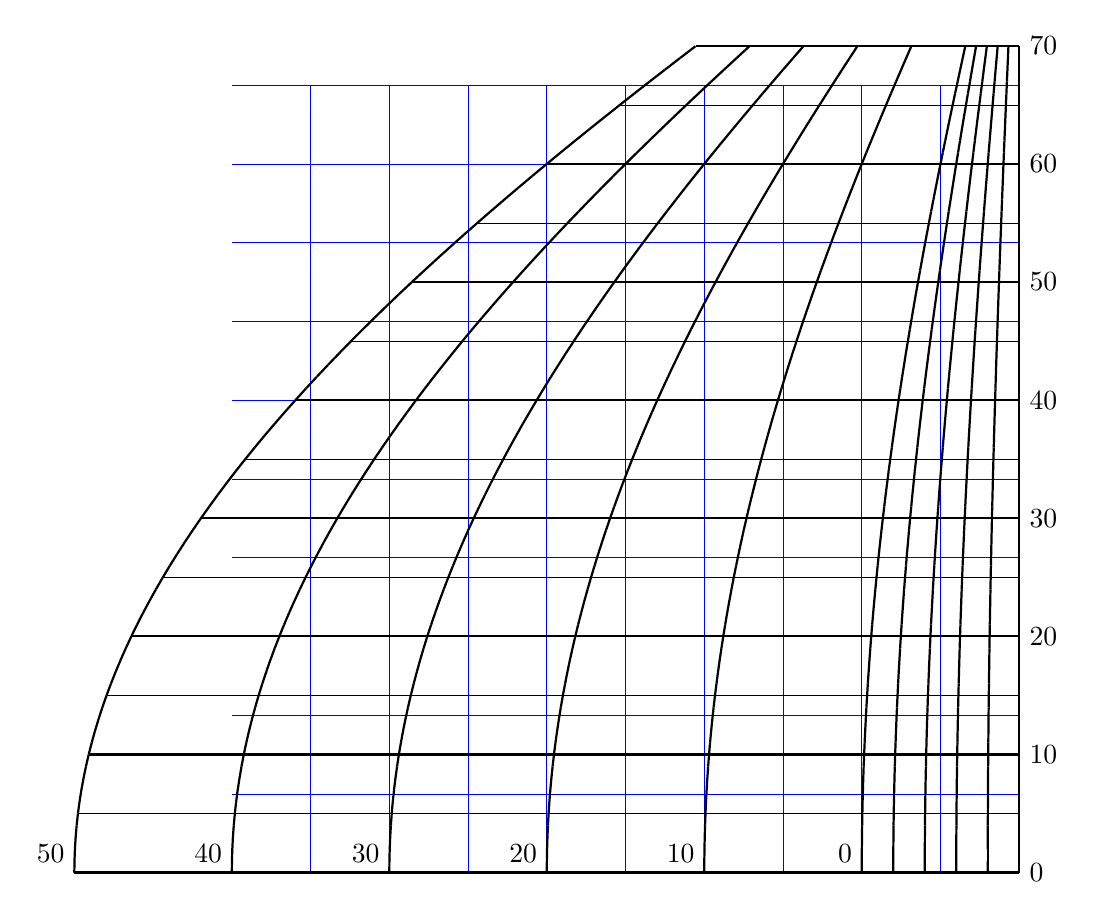
\begin{tikzpicture}[scale=10]
  \def\scalex{2cm};
  \def\scaley{\scalex*0.75};
  \draw[blue,very thin, step=0.1cm] (-1,0) grid (0,1);
  \foreach \step in {0.00,0.02,0.04,0.06,0.08,0.1,0.2,0.3,0.4,0.5,0.6} { %for each of the curved lines
    \foreach \y in {0.0,0.01,...,0.69} {   %for each degree in the vertical scale
      \draw[thick]  ({(-sin(90-\y*100))*\step*\scalex},\y*\scaley) --
      ({(-sin(90-(\y+0.01)*100))*\step*\scalex},{(\y+0.01)*\scaley});
    }
  }
  \foreach \lat in {0, 10,...,70} {  %For each of the horizontal latitude lines
    \draw[thick] ({-sin(90-\lat)*.6*\scalex},\lat/100*\scaley) -- (0,\lat/100*\scaley) node [right] {\lat};
  }
  
  \foreach \lat in {5,15,...,65} {  %For each of the thinner horizontal latitude lines
    \draw[very thin] ({-sin(90-\lat)*.6*\scalex}, \lat/100*\scaley) -- (0,\lat/100*\scaley);
  }
  \foreach \min in {0,10,...,50} {     %For each minute in the latitude scale
    \node [above left] at ({((-\min/10)*(\scalex/10))-(\scalex/10)}, 0) {\min};
    %% \node [above left] at ({-\min/(100-(0.6*\scalex))*\scalex}, 0) {\min};
  }
\end{tikzpicture}

\end{document}
